\documentclass[10pt,a4paper]{article}

\usepackage[utf8]{inputenc}
\usepackage{amsmath, amsfonts, amssymb}
\usepackage{tikz}
\usepackage{pgf}
\usepackage{pgfplots}
\usepackage{hyperref}
\usepackage{comment}
\usepackage{algorithm}
\usepackage[noend]{algpseudocode}
\usepackage{parskip}
\usepackage{listings}
\usepackage{xcolor}
\usepackage{enumerate}
\usepackage[nounderscore]{syntax}

\shortverb{\|}
\setlength{\grammarindent}{2cm}
\newcommand{\indalt}[1][2]{\\\hspace*{#1em}\textbar\quad}

\pgfplotsset{compat=1.3}
\newcommand{\algoname}[1]{\textnormal{\textsc{#1}}}
\title{Implementation and evaluation of the small progress measures algorithm}

\author{Olav Bunte (0803961, o.bunte@student.tue.nl),\\
Maurice Laveaux (0813568, m.laveaux@student.tue.nl),\\
Ziad Ben Snaiba (0748095, z.b.snaiba@student.tue.nl)}

\date{\today}

\begin{document}
\maketitle

\section{Introduction}
This report elaborates on our work and findings of assignment two. The goal of this assignment is to implement and evaluate the small progress measures algorithm as described in \cite{spmpaper}. First we will address the design and implementation of the algorithm in section \ref{design}, along with alternative lifting strategies to make the algorithm more efficient. Then in section \ref{eval} we will show the performance of each lifting strategy using self-made and provided parity games. Lastly, we will reach a conclusion in section \ref{conc}.

\section{Design and implementation}\label{design}
In this section the design and implementation of our small progress measures algorithm is given, which we have programmed using C++. First we will show the data structure
used to store a parity game. Then we elaborate on the design of the small progress measures algorithm itself. Lastly we will show the lifting orders implemented and explain their advantages.

\subsection{Parity Game}
This section contains a description of the expected input and how the parity game is represented as a data structure within the tool.

\subsubsection{Input format}
The parity games are expected to be in an EBNF format \cite{pgsreport}. The tool given here requires a few additional assumption on the input. The names of a vertex are not used in this tool, but can be provided. Additionally, the nodes are expected to be given in ascending order based on their identifier, starting at 0. 

The following slightly adjusted format taken from The PGSolver Collection of Parity Game Solvers \cite{pgsreport} is expected.

\begin{center}
	\begin{minipage}{0.8\linewidth}
		\begin{grammar}
			<parity\_game> ::= [parity <max\_vertex\_id> ;] <node_spec>$^{+}$
			
			<node\_spec> ::= <identifier> <priority> <owner> <successors> [<name>] ;
			
      		<max\_vertex\_id> ::= $\mathbb{N}^+$
      		
      		<identifier> ::= $\mathbb{N}$
      		
      		<priority> ::= $\mathbb{N}$
      		
      		<owner> ::= \textbf{0} | \textbf{1}
      		
      		<successors> ::= <identifier> (, <identifier>)$^{*}$
      		
      		<name> ::= \textquotedblright (any ASCII string not containing \rq \textquotedblright \rq ) \textquotedblright
    \end{grammar}
  \end{minipage}
\end{center}

\subsubsection{Internal representation}
To ensure that look-up times are minimized as much as possible during the solving a bit of pre-processing is done when parsing the parity game. The parity game is represented as a tuple: 

\texttt{ParityGame(Succ, Pred, Prio, PrioCount, MaxPrio, Owner)}, with


\begin{itemize}
	\item \texttt{Succ}: mapping from a vertex to a set of its direct successors,
	\item \texttt{Pred}: mapping from a vertex to a set of its direct, predecessors,
	\item \texttt{Prio}: mapping from a vertex to its priority,
	\item \texttt{PrioCount}: mapping from a priority to how often it occurs in the parity game,
	\item \texttt{MaxPrio}: the maximum priority,
	\item \texttt{Owner}: mapping from a vertex to its owner (even or odd).
\end{itemize}

Given the restrictions on the input given in the previous section all of these can be represented using an array where the index corresponds to the indentifier of the vertex.

\subsection{Small progress measures}
For this algorithm we needed another data structure, namely for progress measures. For this we have chosen to define \texttt{Measure} as a vector of $p$ integers where $p$ is the maximum priority of the parity game plus one. The special progress measure \texttt{TOP} is a vector of only one element, namely the integer 1. The set of possible progress measures for a parity game is also represented by a \texttt{Measure}, holding the maximum possible value for each uneven element.\\
From the definition of a measure, we know that each even index of the measure is always zero. This is used to speed up the creation and comparison of these measures by iterating only over all uneven indices of the measure. Note that because of this we need an extra check to be able to compare to \texttt{TOP}.
\\\\
The small progress measures algorithm is split up in five separate methods:
\begin{itemize}
\item \algoname{getProgressMeasures}: gets the set of all progress measures possible for a given parity game.
\item \algoname{lexicoGreaterThan}: determines whether a \texttt{Measure} is lexicographically greater than another \texttt{Measure}. Can be strict or non-strict and can be tested up to a certain element.
\item \algoname{prog}: computes the value of \textit{Prog} as defined in the slides and in \cite{spmpaper} given a vertex and one of its successors.
\item \algoname{lift}: lifts a vertex as defined in the slides and in \cite{spmpaper}.
\item \algoname{solveParityGame}: the main algorithm itself.\\
\end{itemize}

The pseudo code of the \algoname{getProgressMeasures} method is shown in algorithm \ref{alg:getProgMeas}. This algorithm is relatively simple. It only needs to retrieve the number of vertices with a certain uneven priority, for each uneven priority in the parity game, to get the maximum progress measure possible that is not \texttt{TOP}. This represents the set of all possible progress measures.

\begin{algorithm}
\caption{Get the maximum progress measure}\label{alg:getProgMeas}
\begin{algorithmic}[1]
	\Procedure{getProgressMeasures}{$parityGame$}    
		\State create a the minimal \texttt{Measure} $measure$		
		\ForAll{uneven indices $i$ of $measure$}
			\State $measure[i] = parityGame.getPriorityCount(i)$
		\EndFor
		\State \Return $measure$
	\EndProcedure
\end{algorithmic}
\end{algorithm}

The pseudo code of the \algoname{lexicoGreaterThan} method is shown in algorithm \ref{alg:lexico}. First the cases where at least one of the measures is \texttt{TOP} are taken care of, since it is a special measure. If neither measure equals \texttt{TOP} it iterates over the values of both measures to spot any differences. If it encounters an element in the first measure that is bigger, it knows that it is greater than the second. If it encounters an element in the first measure that is smaller instead, it knows that it is smaller than the second. If they are equal, it checks the next element. If all elements are equal, it will return true or false depending on the value of $strict$.

\begin{algorithm}
\caption{Check lexicographical inequality of two measures}\label{alg:lexico}
\begin{algorithmic}[1]
	\Procedure{lexicoGreaterThan}{$measure1, measure2, strict = true,$ $limit = \infty$}    
		\If{$measure2 == \texttt{TOP}$}
			\If{$measure1 == \texttt{TOP}$}
				\State \Return $\neg strict$
			\Else
				\State \Return $\textit{false}$
			\EndIf
		\Else
			\If{$measure1 == \texttt{TOP}$}
				\State \Return $\textit{true}$
			\Else
				\ForAll{uneven indices $i$ of $measure1$, $i \leq limit$}
					\If{$measure1[i] > measure2[i]$}
						\State \Return $\textit{true}$
					\EndIf
				\EndFor
				\State \Return $\neg strict$
			\EndIf
		\EndIf
	\EndProcedure
\end{algorithmic}
\end{algorithm}

The pseudo code of the \algoname{prog} method is shown in algorithm \ref{alg:prog}. This method is split in two cases: the priority $priority$ of $vertex$ is even or it is uneven.\\
When $priority$ is even, its measure should become the least measure that is lexicographically at least the measure of the successor up to $priority$. This is done by copying all values of the successor to the new measure for $vertex$ up to $priority$ and leaving the rest as zeroes. Note that it does not matter whether the iteration variable $i$ is less than or at most $priority$. Since $priority$ is even it will not be considered in the iteration either way as explained at the start of this section.\\
When $priority$ is uneven, its measure should become the least measure that is lexicographically greater than the measure of the successor up to $priority$. If this is not possible, the measure will be \texttt{TOP}. To do so, we need to copy the measure of the successor to the new measure up to $priority$ and add 1 to the last uneven index, being at most $priority$, where this is possible. This is done by iterating backward over the measure, starting by $priority$. If the value can be incremented, which is tested using $maxMeasures$, it is incremented. Else it is simply copied and the next index is tested. If a previous value has been incremented already, the value is simply copied, since we need the least possible value. If it has not been possible to increment any value, \texttt{TOP} is assigned as the new measure for $vertex$.

\begin{algorithm}
\caption{Compute \textit{Prog}}\label{alg:prog}
\begin{algorithmic}[1]
	\Procedure{prog}{$parityGame, maxMeasures, progressMeasures, vertex, successor$}    
		\State create a the minimal \texttt{Measure} $newMeasure$
		\State $succMeasure = progressMeasures[successor]$
		\State $priority =$ the priority of $vertex$
		\If{$succMeasure == \texttt{TOP}$}
			\State \Return \texttt{TOP}
		\EndIf
		\If{$priority$ is even}
			\ForAll{uneven indices $i$ of $newMeasure$, $i < priority$}
				\State $newMeasure[i] = succMeasure[i]$
			\EndFor
		\Else
			\State $\textit{madeStrictlyGreater} = false$
			\ForAll{uneven indices $i$ of $newMeasure$, from $priority$ to 1}
				\If{$\neg\textit{madeStrictlyGreater}$ and $succMeasure[i] < maxMeasures[i]$}
					\State $newMeasure[i] = succMeasure[i] + 1$
                	\State $\textit{madeStrictlyGreater} = \textit{true}$
                \Else
                	\State $newMeasure[i] = succMeasure[i]$
                \EndIf
            \EndFor
        	\If{$\neg\textit{madeStrictlyGreater}$}
        		\State $newMeasure = \texttt{TOP}$
       		\EndIf
       	\EndIf
       	\State \Return $newMeasure$
	\EndProcedure
\end{algorithmic}
\end{algorithm}

The pseudo code of the \algoname{lift} method is shown in algorithm \ref{alg:lift}. In this method a $vertex$ is lifted. This is done by computing the value of \algoname{prog} for each successor of $vertex$. If $vertex$ is owned by player even these values are minimised, else they 
are maximised.\\
Note that there are some optimisations in this method. If $vertex$ is owned by player even has a self-loop and an even priority, it will always get the minimal measure, since it minimizes all measures at least as big as its successors. Also, since it minimizes, it is no use to keep iterating when the minimal measure has been reached already, so it returns the measure when this is the case. Both optimisations are also present dually if $vertex$ is owned by player odd.

\begin{algorithm}
\caption{Lift a vertex}\label{alg:lift}
\begin{algorithmic}[1]
	\Procedure{lift}{$parityGame, maxMeasures, progressMeasures, vertex$}    
		\State create a \texttt{Measure} $measure$		
		\ForAll{Outgoing vertices $successor$ of $vertex$}
			\State $newMeasure = \algoname{prog}(parityGame, maxMeasures, progressMeasures,$ $vertex, successor)$
			\If{$measure$ has no value}
				\State $measure = newMeasure$
			\EndIf
			\If{$vertex$ is owned by player even}
				\If{$vertex == successor$ and $vertex$ has an even priority}
					\State \Return the minimal \texttt{Measure}
				\EndIf
				\If{$\algoname{lexicoGreaterThan}(measure, newMeasure)$}
					\State $measure = newMeasure$
				\EndIf
				\If{$measure$ is the minimal measure}
					\State \Return $measure$
				\EndIf
			\Else
				\If{$vertex == successor$ and $vertex$ has an uneven priority}
					\State \Return \texttt{TOP}
				\EndIf
				\If{$\algoname{lexicoGreaterThan}(newMeasure, measure)$}
					\State $measure = newMeasure$
				\EndIf
				\If{$measure == \texttt{TOP}$}
					\State \Return $\texttt{TOP}$
				\EndIf
			\EndIf
		\EndFor
		\State \Return $measure$
	\EndProcedure
\end{algorithmic}
\end{algorithm}

The pseudo code of the \algoname{solveParityGame} method is shown in algorithm \ref{alg:solve}. This is the main method: this is where the algorithm starts and ends. After getting the set of possible progress measures, it will lift all vertices in a given order. When the measure of a vertex has increased, a boolean $increased$ will be set to true to notify that the list of progress measures has increased in this loop over the order. When all vertices in the order have been lifted and $increased$ is true, it will start a new lift loop over the order. The algorithm keeps doing this until $increased$ is no longer true after a lift loop, meaning that the progress measures have been converged. When this is the case, it can check which vertices are won by which player. If a vertex as \texttt{TOP} as its final measure, player odd has won this vertex. If the measure a different value than \texttt{TOP} this vertex is won by player even.

\begin{algorithm}
\caption{The main method of solving a parity game}\label{alg:solve}
\begin{algorithmic}[1]
	\Procedure{solveParityGame}{$paritygame, vertexOrder$}    
		\State Initialize $progressMeasures$ with the minimal \texttt{Measure} for each vertex
		\State $maxMeasures$ = $\algoname{getProgressMeasures}(paritygame)$
		\State create boolean $increased$
		\Repeat
			\State $increased = \textit{false}$
			\For{all vertices $vertex$ in the $vertexOrder$}
				\State $measure = progressMeasures(vertex)$
				\State $newMeasure = \algoname{lift}(parityGame, maxMeasures, progressMeasures, vertex)$
				\If{$\algoname{lexicoGreaterThan}(newMeasure, measure)$}
					\State $progressMeasures[vertex] = newMeasures$
					\State $increased = true$
				\EndIf
			\EndFor
		\Until{$\neg increased$}
		\For{all vertices $vertex$}
			\If{$progressMeasures[vertex] == \texttt{TOP}$}
				\State $vertex$ is won by player odd
			\Else
				\State $vertex$ is won by player even
			\EndIf
		\EndFor
	\EndProcedure
\end{algorithmic}
\end{algorithm}

\subsection{Lifting orders}
As can be seen in \ref{alg:solve}, the vertices are lifted in a certain order. We have implemented five orders in total, two of which are given in the assignment and three of which we have created ourselves. Below are all the implemented orders given with their explanation and advantages.

\subsubsection{Input}
This lifting order simply iterates over the vertices in the order of the input, starting by 0 and incrementing by one every vertex. There is no real advantage or rationale behind this order, except that it is deterministic and it is easy to compute.

\subsubsection{Random}
This lifting order, as the name suggests, uses a random ordering of all vertices. This ordering is set at the start of the execution of the algorithm.\\
The randomness causes the algorithm to be non-deterministic, giving different execution times every execution. This can, depending on the created order, either be an advantage or a disadvantage. It can happen that in one execution the order is very efficient and in another execution it is very inefficient.

\subsubsection{In degree}\label{indegree}
This lifting order is based on the fact that the \texttt{prog} method takes the measure of a successor vertex and either tries to increase it or copy it. In this order all vertices are descendingly ordered on their in degree (the amount of incoming edges). Since \texttt{prog} uses successors to create a measure, more vertices will have profit in the same iteration over the order when first lifting a vertex with a higher in degree than when first lifting a vertex with a lower in degree.


This order works well with parity games with a big varying in degree for the nodes. Especially parity games with a star-like form, where many vertices point to one vertex, have profit form this order. In such a case the vertex in the center of the star will be lifted first. Afterwards the vertices on the points of the star will be lifted, profiting form the lifted center vertex.

\subsubsection{Breadth first search}
% Explanation
Like the previous order, this lifting order is based on the fact that the \texttt{prog} method takes the measure of a successor vertex and either tries to increase it or copy it. When this successor vertex was already lifted beforehand the resulting measure for the lifted vertex will be even higher. So a breadth first search that places a vertex before its predecessors can possibly increase performance. It is not always possible to get all vertices starting from a single position, thus when the order is not complete the next smallest vertex is selected and another breadth first search is conducted. The implementation code is included in the appendix under \ref{appendix:bfs}.

% Optimal example
An example where this order is more efficient then the others is a single cycle where every vertex has a neighbour as successor. The input order doesn't have to follow the cycle reversed and the in-degree is the same for all vertices. So in this case the breadth first search will put the vertices in reversed order and the measures will be lifted faster.\\
Note that this order is not necessarily better in the example parity game given for the in degree. For example, if the center vertex of the star is the last vertex in the input, the order is actually quite bad. This gave us the idea of creating a fifth lifting order.

\subsubsection{Breadth first search with in degree order}
This lifting order combines the advantages and rationale of the two orders above. It first creates the in degree order as described in section \ref{indegree}. Then it uses the first vertex in this order to start the first breadth first search. When the search cannot go any further but there are vertices left, it will start a new search from the first vertex in the in degree order that hasn't been found yet.

\section{Evaluation}\label{eval}

In the evaluation the blue line represents the input order, red represents the random order, ?? represents the indegree order and ?? represents the breadth first order.

\subsection{Self-made parity games}

Resulting partitions for the sets.

\begin{enumerate}[01]
	\item Even set \{0, 1\}, Odd set \{2, 3, 4, 5, 6\}
	\item Odd set \{0, 1, 2, 3, 4, 5, 6, 7, 8\}
	\item Even set \{0, 1, 3, 7\}, Odd set \{2, 4, 5, 6\}
	\item Odd set \{0, 1, 2, 3, 4, 5\}
	\item Odd set \{0, 1, 2, 3, 4, 5\}

\end{enumerate}

The performance measures over 100 iterations, mainly used for the random order, but still done on every order for consistency.

\begin{tabular}{l l l l l}
	Game	& Input	 & Random & Indegree & Breadthfirst \\
	01		& 0.0018 & 0.0017 & 0.0019   & 0.0018 \\
	02		& 0.0019 & 0.0019 & 0.0019   & 0.0018 \\
	03		& 0.0018 & 0.0019 & 0.0018 	 & 0.0018 \\
	04		& 0.0018 & 0.0019 & 0.0020	 & 0.0017 \\
	05		& 0.0018 & 0.0017 & 0.0019	 & 0.0018 

\end{tabular}

\subsection{Dining Philosophers}

\subsubsection{Invariantly inevitably eat}

The first vertex is won by odd.

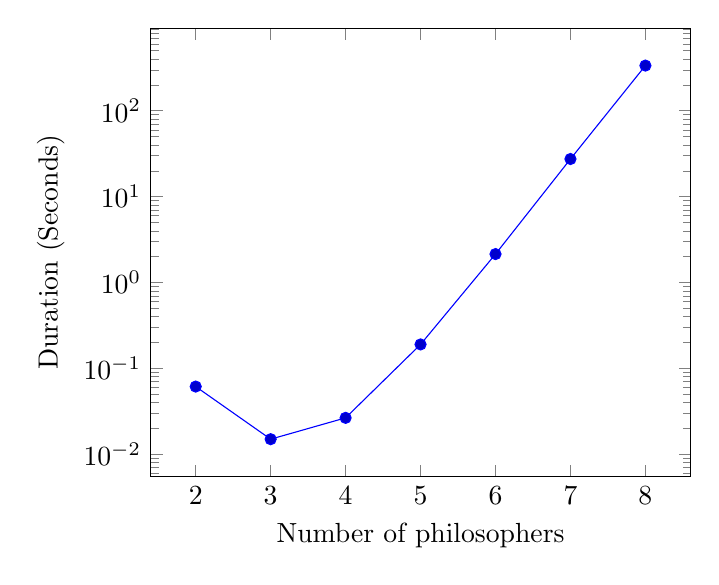
\begin{tikzpicture}
  	\begin{axis}[ 
    	xlabel={Number of philosophers},
    	ylabel={Duration (Seconds)},
    	ymode=log,
        log basis y={10}
  	] 
    \addplot+ [color=blue] coordinates { (2, 0.0615) (3, 0.015) (4, 0.02658) (5, 0.1903) (6, 2.145) (7, 27.434) (8, 335.774) };
  	\end{axis}
\end{tikzpicture}

\subsubsection{Invariantly possibly eat}

The first vertex is won by odd.

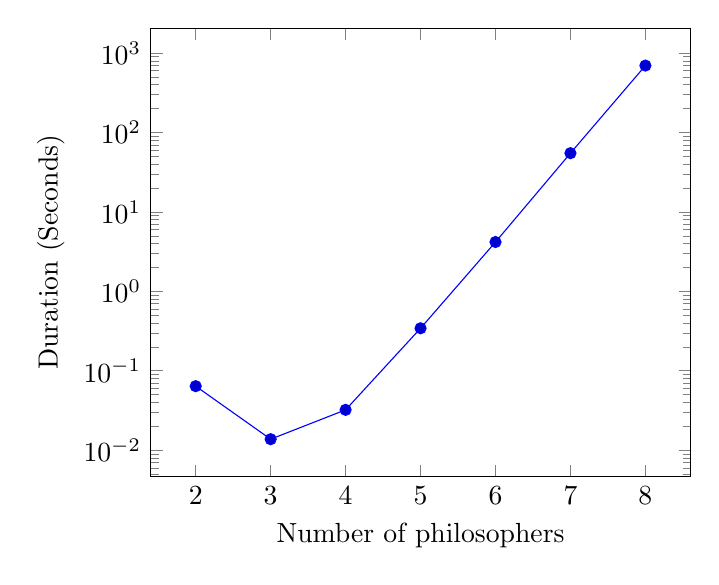
\begin{tikzpicture}
  	\begin{axis}[ 
    	xlabel={Number of philosophers},
    	ylabel={Duration (Seconds)},
    	ymode=log,
        log basis y={10}
  	] 
    \addplot+ [color=blue] coordinates { (2, 0.06396) (3, 0.013748) (4, 0.0322) (5, 0.3428) (6, 4.18) (7, 54.96) (8, 696.657) };
  	\end{axis}
\end{tikzpicture}

\subsubsection{Invariantly plato starves}

The first vertex is won by odd. 

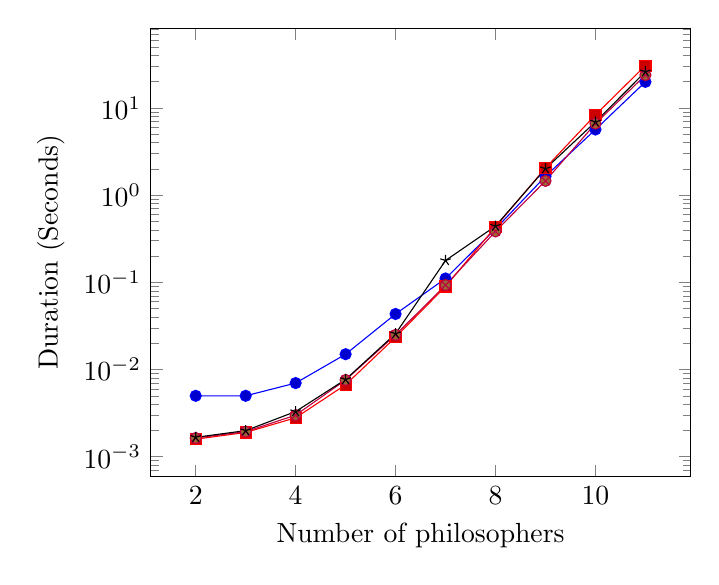
\begin{tikzpicture}
  	\begin{axis}[ 
    	xlabel={Number of philosophers},
    	ylabel={Duration (Seconds)},
    	ymode=log,
        log basis y={10}
  	] 
    \addplot+ [color=blue] coordinates { (2, 0.005) (3, 0.005) (4, 0.007) (5, 0.015) (6, 0.0434) (7, 0.11081) (8, 0.4102) (9, 1.649) (10, 5.664) (11, 19.9487) };
        
    \addplot+ [color=red] coordinates { (2, 0.00159) (3, 0.0019) (4, 0.0028) (5, 0.0067) (6, 0.0235) (7, 0.0898) (8, 0.4324) (9, 2.0533) (10, 8.333) (11, 30.65) };
        
    \addplot+ [color=purple] coordinates { (2, 0.00164) (3, 0.00194) (4, 0.003) (5, 0.0076) (6, 0.025) (7, 0.093) (8, 0.384) (9, 1.458) (10, 6.6211) (11, 23.879)};
    
    \addplot+ [color=black] coordinates { (2, 0.00167) (3, 0.001994) (4, 0.0033) (5, 0.0077) (6, 0.0258) (7, 0.1782) (8, 0.442) (9, 2.013) (10, 6.923) (11, 26.045)};
  	\end{axis}
\end{tikzpicture}

\subsubsection{Plato infinitely often can eat}

The first vertex is won by odd.

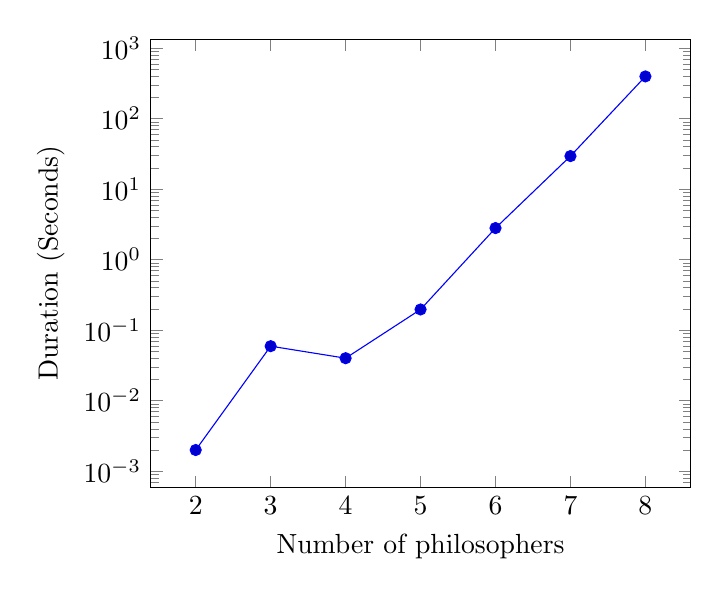
\begin{tikzpicture}
  	\begin{axis}[ 
    	xlabel={Number of philosophers},
    	ylabel={Duration (Seconds)},
    	ymode=log,
        log basis y={10}
  	] 
    \addplot+ [color=blue] coordinates { (2, 0.002) (3, 0.0594) (4, 0.0401) (5, 0.1970) (6, 2.8098) (7, 29.4722) (8, 397.45) };
  	\end{axis}
\end{tikzpicture}

\subsection{Elevator}

\subsubsection{1 elevator}

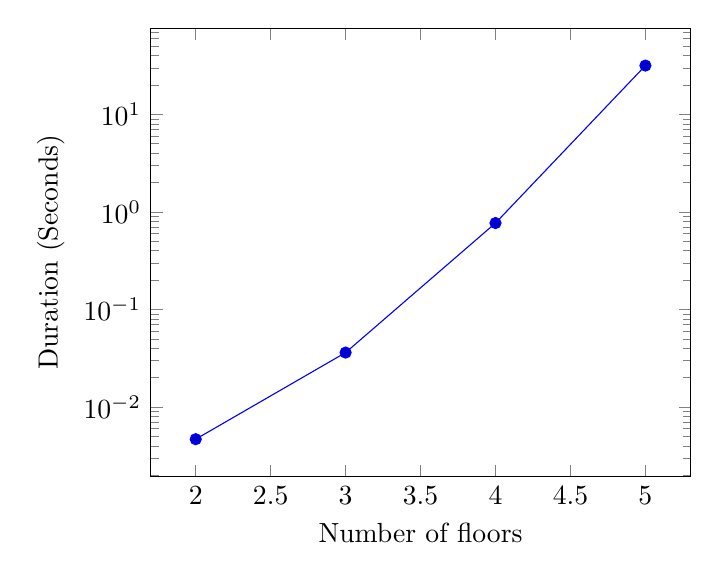
\begin{tikzpicture}
  	\begin{axis}[ 
    	xlabel={Number of floors},
    	ylabel={Duration (Seconds)},
    	ymode=log,
        log basis y={10}
  	] 
    \addplot+ [color=blue] coordinates { (2, 0.00468) (3, 0.03615) (4, 0.769) (5, 31.619) };
  	\end{axis}
\end{tikzpicture}

\section{Conclusion}\label{conc}


\begin{thebibliography}{9}
\bibitem{spmpaper} M. Jurdzi\'{n}ski: Small Progress Measures for Solving Parity Games, March 2000
\bibitem{pgsreport} O. Friedmann and Martin Lange: The PGSolver Collection of Parity Game Solvers, March 2014
\end{thebibliography}


\newpage
\appendix

\section{Breadth first order}\label{appendix:bfs}

\begin{verbatim}
// Create the order and coloring vectors.
order = std::vector<Vertex>(parityGame.getNumberOfVertices(), -1);
std::vector<int> graphColoring(parityGame.getNumberOfVertices());

// The queue for to be handled vertices.
std::queue<Vertex> workQueue;

// The current order being search and vertex beind handled.
int ordering = 0;
Vertex currentVertex = 0;

while (ordering != parityGame.getNumberOfVertices()) {
	workQueue.push(currentVertex); // Add the first vertex.

    while (!workQueue.empty()) {
    	// Pop the first element.
        Vertex current = workQueue.front(); workQueue.pop();

        if (graphColoring[current] == 0) {
        	// If the color is not yet set .
            for (auto& incomingVertex : parityGame.getIncomingVertices(current)) {
            	workQueue.push(incomingVertex);
            }

            // Color the current vertex.
            graphColoring[current] = 1;
            order[ordering++] = current;
        }
    }

    // Select the smallest vertex not yet put into ordering.
    for (Vertex current = 0; current < graphColoring.size(); ++current) {
    	if (graphColoring[current] == 0) {
        	currentVertex = current;
            break;
        }
    }
}
\end{verbatim}






\end{document}